% ============================================================
\chapter{Apprentissage bay\'esien}
\label{ch:bayesien}
\index{apprentissage bay\'esien}
% ============================================================

\section{Inf\'erence bay\'esienne}
\label{sec:inference}
\index{inf\'erence bay\'esienne}

\subsection{Le th\'eor\`eme de Bayes}

\begin{theoreme}[Th\'eor\`eme de Bayes]
Soit $\bm{\theta}$ le vecteur de param\`etres et $\mathcal{D}$ les donn\'ees
observ\'ees. La \textbf{distribution a posteriori} est~:
\begin{equation}
  \underbrace{p(\bm{\theta} \mid \mathcal{D})}_{\text{post\'erieur}} =
  \frac{\overbrace{p(\mathcal{D} \mid \bm{\theta})}^{\text{vraisemblance}}
  \cdot \overbrace{p(\bm{\theta})}^{\text{prior}}}
  {\underbrace{p(\mathcal{D})}_{\text{\'evidence}}}
  \label{eq:bayes}
\end{equation}
o\`u $p(\mathcal{D}) = \int p(\mathcal{D} \mid \bm{\theta})\,
p(\bm{\theta})\, d\bm{\theta}$ est la vraisemblance marginale.
\end{theoreme}

\begin{center}
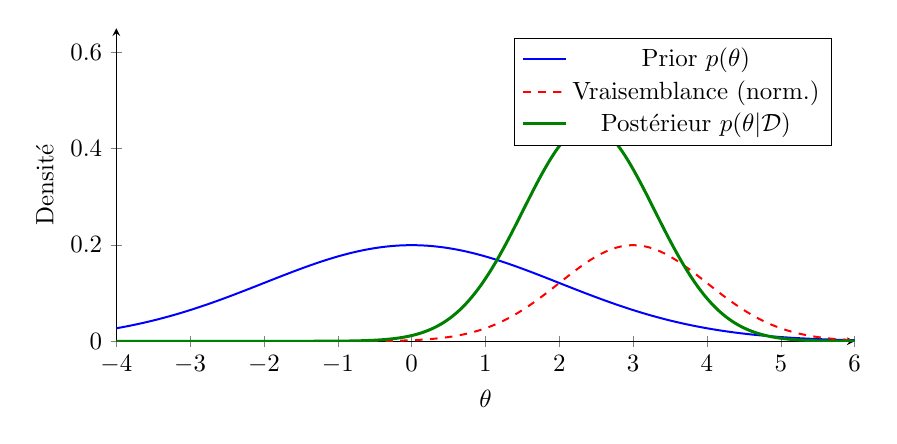
\begin{tikzpicture}[scale=0.9]
  \begin{axis}[
    width=12cm, height=6cm,
    xlabel={$\theta$},
    ylabel={Densit\'e},
    xmin=-4, xmax=6, ymin=0, ymax=0.65,
    legend pos=north east,
    axis lines=left,
    every axis plot/.append style={thick, samples=100, smooth}
  ]
    % Prior
    \addplot[blue, domain=-4:6]
      {exp(-(x-0)^2/(2*2^2)) / (2*sqrt(2*pi))};
    \addlegendentry{Prior $p(\theta)$}
    % Likelihood (scaled)
    \addplot[red, dashed, domain=-4:6]
      {exp(-(x-3)^2/(2*1^2)) / (1*sqrt(2*pi)) * 0.5};
    \addlegendentry{Vraisemblance (norm.)}
    % Posterior
    \addplot[green!50!black, very thick, domain=-4:6]
      {exp(-(x-2.4)^2/(2*0.89^2)) / (0.89*sqrt(2*pi))};
    \addlegendentry{Post\'erieur $p(\theta|\mathcal{D})$}
  \end{axis}
\end{tikzpicture}
\end{center}

\begin{intuition}[title=\textbf{Interpr\'etation}]
\begin{itemize}
  \item Le \textbf{prior} $p(\bm{\theta})$ encode nos croyances avant
    d'observer les donn\'ees.
  \item La \textbf{vraisemblance} $p(\mathcal{D} \mid \bm{\theta})$ mesure
    la compatibilit\'e des donn\'ees avec les param\`etres.
  \item Le \textbf{post\'erieur} $p(\bm{\theta} \mid \mathcal{D})$ combine
    les deux~: il est un compromis entre prior et donn\'ees.
  \item Plus on a de donn\'ees, plus le post\'erieur est domin\'e par la
    vraisemblance.
\end{itemize}
\end{intuition}

\subsection{MAP vs MLE}
\index{MAP}\index{MLE}

\begin{definition}[Maximum de vraisemblance (MLE)]
L'estimateur du \textbf{maximum de vraisemblance} est~:
\begin{equation}
  \hat{\bm{\theta}}_{\text{MLE}} = \argmax_{\bm{\theta}}\;
  p(\mathcal{D} \mid \bm{\theta}) = \argmax_{\bm{\theta}}
  \sum_{i=1}^n \ln p(\bm{x}_i \mid \bm{\theta})
\end{equation}
\end{definition}

\begin{definition}[Maximum a posteriori (MAP)]
L'estimateur \textbf{MAP} int\`egre le prior~:
\begin{equation}
  \hat{\bm{\theta}}_{\text{MAP}} = \argmax_{\bm{\theta}}\;
  p(\bm{\theta} \mid \mathcal{D}) = \argmax_{\bm{\theta}}
  \left[\ln p(\mathcal{D} \mid \bm{\theta}) + \ln p(\bm{\theta})\right]
  \label{eq:map}
\end{equation}
\end{definition}

\begin{proposition}[MAP et r\'egularisation]
L'estimation MAP avec un prior gaussien $p(\bm{\theta}) =
\mathcal{N}(\bm{0}, \tau^2 \bm{I})$ est \'equivalente \`a la r\'egularisation
$L_2$ (Ridge)~:
\begin{equation}
  \hat{\bm{\theta}}_{\text{MAP}} = \argmin_{\bm{\theta}} \left[
  -\ln p(\mathcal{D} \mid \bm{\theta}) + \frac{1}{2\tau^2}
  \norm{\bm{\theta}}^2 \right]
\end{equation}
De m\^eme, un prior Laplacien donne la r\'egularisation $L_1$ (Lasso).
\end{proposition}

\begin{attention}[title=\textbf{MAP $\neq$ bay\'esien complet}]
L'estimation MAP fournit une estimation \emph{ponctuelle} de $\bm{\theta}$.
L'approche bay\'esienne compl\`ete utilise la distribution \emph{enti\`ere}
du post\'erieur, ce qui permet de quantifier l'incertitude.
\end{attention}

% ============================================================
\section{Priors conjugu\'es}
\label{sec:conjugues}
\index{prior conjugu\'e}
% ============================================================

\begin{definition}[Famille conjugu\'ee]
Une famille de priors $\mathcal{F}$ est \textbf{conjugu\'ee} pour une
vraisemblance donn\'ee si le post\'erieur appartient \'egalement \`a
$\mathcal{F}$~:
\begin{equation}
  p(\bm{\theta}) \in \mathcal{F} \quad \Longrightarrow \quad
  p(\bm{\theta} \mid \mathcal{D}) \in \mathcal{F}
\end{equation}
\end{definition}

\begin{formules}[title=\textbf{Exemples de priors conjugu\'es}]
\begin{center}
\renewcommand{\arraystretch}{1.3}
\begin{tabular}{lll}
  \toprule
  \textbf{Vraisemblance} & \textbf{Prior conjugu\'e} & \textbf{Post\'erieur} \\
  \midrule
  Bernoulli$(p)$ & Beta$(\alpha, \beta)$ &
    Beta$(\alpha + s, \beta + n - s)$ \\
  Poisson$(\lambda)$ & Gamma$(\alpha, \beta)$ &
    Gamma$(\alpha + s, \beta + n)$ \\
  $\mathcal{N}(\mu, \sigma^2$ connu$)$ &
    $\mathcal{N}(\mu_0, \sigma_0^2)$ &
    $\mathcal{N}(\mu_n, \sigma_n^2)$ \\
  $\mathcal{N}(\mu$ connu$, \sigma^2)$ &
    Inv-Gamma$(\alpha, \beta)$ &
    Inv-Gamma$(\alpha', \beta')$ \\
  \bottomrule
\end{tabular}
\end{center}
\end{formules}

\begin{exemple}[Mod\`ele gaussien avec variance connue]
Soit $x_1, \ldots, x_n \overset{\text{i.i.d.}}{\sim}
\mathcal{N}(\mu, \sigma^2)$ avec $\sigma^2$ connu et prior
$\mu \sim \mathcal{N}(\mu_0, \sigma_0^2)$. Le post\'erieur est~:
\begin{equation}
  \mu \mid \mathcal{D} \sim \mathcal{N}(\mu_n, \sigma_n^2)
\end{equation}
avec~:
\begin{align}
  \sigma_n^2 &= \left(\frac{1}{\sigma_0^2} + \frac{n}{\sigma^2}\right)^{-1}
  \label{eq:post-var} \\
  \mu_n &= \sigma_n^2 \left(\frac{\mu_0}{\sigma_0^2} +
  \frac{n\bar{x}}{\sigma^2}\right)
  \label{eq:post-mean}
\end{align}
o\`u $\bar{x} = \frac{1}{n}\sum_{i=1}^n x_i$. On note que $\mu_n$ est une
moyenne pond\'er\'ee entre le prior $\mu_0$ et la moyenne empirique $\bar{x}$.
\end{exemple}

% ============================================================
\section{R\'egression lin\'eaire bay\'esienne}
\label{sec:blr}
\index{r\'egression lin\'eaire bay\'esienne}
% ============================================================

\subsection{Mod\`ele}

On consid\`ere le mod\`ele lin\'eaire~:
\begin{equation}
  y_i = \bm{w}^\top \bm{x}_i + \varepsilon_i, \quad
  \varepsilon_i \sim \mathcal{N}(0, \sigma^2)
\end{equation}
soit en forme matricielle $\bm{y} = \bm{X}\bm{w} + \bm{\varepsilon}$ avec
$\bm{X} \in \R^{n \times d}$.

\subsection{Prior et post\'erieur}

\begin{formules}[title=\textbf{R\'egression lin\'eaire bay\'esienne --- D\'erivation compl\`ete}]
\textbf{Prior~:} $\bm{w} \sim \mathcal{N}(\bm{m}_0, \bm{S}_0)$.

\textbf{Vraisemblance~:}
\begin{equation}
  p(\bm{y} \mid \bm{X}, \bm{w}) = \mathcal{N}(\bm{y} \mid \bm{X}\bm{w},
  \sigma^2 \bm{I}_n) = \prod_{i=1}^n \mathcal{N}(y_i \mid \bm{w}^\top
  \bm{x}_i, \sigma^2)
\end{equation}

\textbf{Post\'erieur~:} par conjugaison gaussienne~:
\begin{equation}
  p(\bm{w} \mid \bm{X}, \bm{y}) = \mathcal{N}(\bm{w} \mid \bm{m}_n,
  \bm{S}_n)
  \label{eq:blr-posterior}
\end{equation}
avec~:
\begin{align}
  \bm{S}_n &= \left(\bm{S}_0^{-1} + \frac{1}{\sigma^2}\bm{X}^\top
  \bm{X}\right)^{-1}
  \label{eq:blr-Sn} \\
  \bm{m}_n &= \bm{S}_n \left(\bm{S}_0^{-1}\bm{m}_0 +
  \frac{1}{\sigma^2}\bm{X}^\top \bm{y}\right)
  \label{eq:blr-mn}
\end{align}
\end{formules}

\begin{proof}
La log-densit\'e du post\'erieur (aux constantes pr\`es) est~:
\begin{align}
  \ln p(\bm{w} \mid \bm{X}, \bm{y}) &\propto \ln p(\bm{y} \mid \bm{X},
  \bm{w}) + \ln p(\bm{w}) \\
  &= -\frac{1}{2\sigma^2}\norm{\bm{y} - \bm{X}\bm{w}}^2 -
  \frac{1}{2}(\bm{w} - \bm{m}_0)^\top \bm{S}_0^{-1}(\bm{w} - \bm{m}_0)
  + \text{cst}
\end{align}
En d\'eveloppant les termes quadratiques en $\bm{w}$ et en compl\'etant le
carr\'e~:
\begin{align}
  &= -\frac{1}{2}\bm{w}^\top\!\underbrace{\left(\bm{S}_0^{-1} +
  \frac{1}{\sigma^2}\bm{X}^\top\bm{X}\right)}_{\bm{S}_n^{-1}}\!\bm{w}
  + \bm{w}^\top\!\underbrace{\left(\bm{S}_0^{-1}\bm{m}_0 +
  \frac{1}{\sigma^2}\bm{X}^\top\bm{y}\right)}_{\bm{S}_n^{-1}\bm{m}_n}
  + \text{cst}
\end{align}
On reconna\^it une forme quadratique gaussienne
$\mathcal{N}(\bm{m}_n, \bm{S}_n)$.
\end{proof}

\begin{remarque}
Avec le prior $\bm{m}_0 = \bm{0}$ et $\bm{S}_0 = \tau^2 \bm{I}$, la moyenne
du post\'erieur co\"incide avec la solution Ridge~:
\begin{equation}
  \bm{m}_n = \left(\bm{X}^\top\bm{X} + \frac{\sigma^2}{\tau^2}
  \bm{I}\right)^{-1}\bm{X}^\top\bm{y}
\end{equation}
\end{remarque}

\subsection{Distribution pr\'edictive}

\begin{definition}[Distribution pr\'edictive]
Pour un nouveau point $\bm{x}_*$, la \textbf{distribution pr\'edictive}
int\`egre sur tous les param\`etres possibles~:
\begin{equation}
  p(y_* \mid \bm{x}_*, \mathcal{D}) = \int p(y_* \mid \bm{x}_*, \bm{w})\,
  p(\bm{w} \mid \mathcal{D})\, d\bm{w}
\end{equation}
\end{definition}

\begin{theoreme}[Pr\'ediction bay\'esienne lin\'eaire]
La distribution pr\'edictive est gaussienne~:
\begin{equation}
  p(y_* \mid \bm{x}_*, \mathcal{D}) = \mathcal{N}(y_* \mid \bm{m}_n^\top
  \bm{x}_*, \; \sigma_*^2)
  \label{eq:blr-predictive}
\end{equation}
avec~:
\begin{equation}
  \sigma_*^2 = \sigma^2 + \bm{x}_*^\top \bm{S}_n \bm{x}_*
\end{equation}
Le premier terme $\sigma^2$ est le bruit al\'eatoire et le second
$\bm{x}_*^\top \bm{S}_n \bm{x}_*$ est l'\textbf{incertitude \'epist\'emique}
(li\'ee au manque de donn\'ees).
\end{theoreme}

% ============================================================
\section{Processus gaussiens}
\label{sec:gp}
\index{processus gaussien}
% ============================================================

\subsection{D\'efinition}

\begin{definition}[Processus gaussien]
Un \textbf{processus gaussien} (GP) est une collection de variables al\'eatoires
dont toute sous-collection finie suit une distribution gaussienne jointe.
Un GP est enti\`erement d\'efini par~:
\begin{itemize}
  \item une fonction de moyenne $m(\bm{x}) = \E[f(\bm{x})]$,
  \item une fonction de covariance (noyau)
    $\kappa(\bm{x}, \bm{x}') = \Cov[f(\bm{x}), f(\bm{x}')]$.
\end{itemize}
On note $f \sim \mathcal{GP}(m, \kappa)$.
\end{definition}

\subsection{Fonctions noyau}
\index{noyau!fonction}

\begin{formules}[title=\textbf{Noyaux courants}]
\begin{align}
  \text{RBF (SE)~:} \quad & \kappa(\bm{x}, \bm{x}') = \sigma_f^2
  \exp\!\left(-\frac{\norm{\bm{x} - \bm{x}'}^2}{2\ell^2}\right)
  \label{eq:rbf} \\
  \text{Mat\'ern $\nu = 3/2$~:} \quad & \kappa(\bm{x}, \bm{x}') =
  \sigma_f^2 \left(1 + \frac{\sqrt{3}\,r}{\ell}\right)
  \exp\!\left(-\frac{\sqrt{3}\,r}{\ell}\right)
  \label{eq:matern32} \\
  \text{P\'eriodique~:} \quad & \kappa(\bm{x}, \bm{x}') = \sigma_f^2
  \exp\!\left(-\frac{2\sin^2(\pi\norm{\bm{x}-\bm{x}'}/p)}{\ell^2}\right)
  \label{eq:periodic} \\
  \text{Lin\'eaire~:} \quad & \kappa(\bm{x}, \bm{x}') = \sigma_f^2\,
  \bm{x}^\top \bm{x}'
  \label{eq:linear}
\end{align}
o\`u $r = \norm{\bm{x} - \bm{x}'}$, $\ell$ est la longueur
caract\'eristique, $\sigma_f^2$ la variance du signal.
\end{formules}

\begin{intuition}[title=\textbf{R\^ole des hyperparam\`etres}]
\begin{itemize}
  \item $\ell$ (longueur caract\'eristique)~: contr\^ole la <<~rugosit\'e~>>
    de la fonction. Grand $\ell$ $\Rightarrow$ fonctions lisses.
  \item $\sigma_f^2$ (variance du signal)~: contr\^ole l'amplitude des
    variations.
  \item $\sigma_n^2$ (bruit)~: variance du bruit d'observation.
\end{itemize}
\end{intuition}

\subsection{R\'egression par processus gaussien}
\index{r\'egression!processus gaussien}

Soit $\mathcal{D} = \{(\bm{x}_i, y_i)\}_{i=1}^n$ avec
$y_i = f(\bm{x}_i) + \varepsilon_i$, $\varepsilon_i \sim
\mathcal{N}(0, \sigma_n^2)$.

\begin{formules}[title=\textbf{R\'egression GP --- Formules pr\'edictives}]
Pour un ensemble de points test $\bm{X}_*$, la distribution pr\'edictive
est~:
\begin{equation}
  \bm{f}_* \mid \bm{X}_*, \bm{X}, \bm{y} \sim
  \mathcal{N}(\bar{\bm{f}}_*, \Cov(\bm{f}_*))
\end{equation}
avec~:
\begin{align}
  \bar{\bm{f}}_* &= \bm{K}_*^\top (\bm{K} + \sigma_n^2 \bm{I})^{-1} \bm{y}
  \label{eq:gp-mean} \\
  \Cov(\bm{f}_*) &= \bm{K}_{**} - \bm{K}_*^\top (\bm{K} + \sigma_n^2
  \bm{I})^{-1} \bm{K}_*
  \label{eq:gp-cov}
\end{align}
o\`u $\bm{K} = \kappa(\bm{X}, \bm{X}) \in \R^{n \times n}$,
$\bm{K}_* = \kappa(\bm{X}, \bm{X}_*) \in \R^{n \times n_*}$,
$\bm{K}_{**} = \kappa(\bm{X}_*, \bm{X}_*) \in \R^{n_* \times n_*}$.
\end{formules}

\begin{proof}[D\'erivation]
Par d\'efinition du GP, la distribution jointe est~:
\begin{equation}
  \begin{pmatrix} \bm{y} \\ \bm{f}_* \end{pmatrix} \sim
  \mathcal{N}\!\left(\bm{0},
  \begin{pmatrix}
    \bm{K} + \sigma_n^2\bm{I} & \bm{K}_* \\
    \bm{K}_*^\top & \bm{K}_{**}
  \end{pmatrix}\right)
\end{equation}
Par la formule de conditionnement gaussien, si
$\begin{pmatrix} \bm{a} \\ \bm{b} \end{pmatrix} \sim
\mathcal{N}\!\left(\bm{0},
\begin{pmatrix} \bm{A} & \bm{C} \\ \bm{C}^\top & \bm{B}
\end{pmatrix}\right)$, alors~:
\begin{equation}
  \bm{b} \mid \bm{a} \sim \mathcal{N}(\bm{C}^\top \bm{A}^{-1}\bm{a},\;
  \bm{B} - \bm{C}^\top \bm{A}^{-1}\bm{C})
\end{equation}
L'application directe donne les \'equations~\eqref{eq:gp-mean}
et~\eqref{eq:gp-cov}.
\end{proof}

\subsection{Optimisation des hyperparam\`etres}

\begin{definition}[Log-vraisemblance marginale]
Les hyperparam\`etres $\bm{\phi} = (\ell, \sigma_f, \sigma_n)$ sont optimis\'es
par maximisation de la log-vraisemblance marginale~:
\begin{equation}
  \ln p(\bm{y} \mid \bm{X}, \bm{\phi}) = -\frac{1}{2}\bm{y}^\top
  (\bm{K} + \sigma_n^2\bm{I})^{-1}\bm{y} - \frac{1}{2}\ln|\bm{K} +
  \sigma_n^2\bm{I}| - \frac{n}{2}\ln(2\pi)
  \label{eq:gp-lml}
\end{equation}
Les trois termes repr\'esentent respectivement l'ajustement aux donn\'ees,
la p\'enalit\'e de complexit\'e, et une constante de normalisation.
\end{definition}

\begin{center}
\begin{tikzpicture}[scale=0.85]
  \begin{axis}[
    width=12cm, height=7cm,
    xlabel={$x$},
    ylabel={$f(x)$},
    xmin=-5, xmax=5, ymin=-3, ymax=3,
    legend pos=north west,
    axis lines=left
  ]
    % Mean prediction
    \addplot[blue, very thick, domain=-5:5, samples=100]
      {sin(deg(x)) * exp(-0.1*x^2)};
    \addlegendentry{Moyenne $\bar{f}_*$}
    % Uncertainty band
    \addplot[name path=upper, blue!20, domain=-5:5, samples=100]
      {sin(deg(x))*exp(-0.1*x^2) + 0.3 + 0.15*abs(x)};
    \addplot[name path=lower, blue!20, domain=-5:5, samples=100]
      {sin(deg(x))*exp(-0.1*x^2) - 0.3 - 0.15*abs(x)};
    \addplot[blue!20, fill opacity=0.5] fill between[of=upper and lower];
    \addlegendentry{$\pm 2\sigma$ (incertitude)}
    % Training points
    \addplot[only marks, mark=*, mark size=2.5pt, red]
      coordinates {(-3, -0.1) (-2, -0.6) (-1, -0.7) (0, 0.1)
                   (1, 0.8) (2, 0.5) (3, -0.05)};
    \addlegendentry{Donn\'ees}
  \end{axis}
\end{tikzpicture}
\end{center}

% ============================================================
\section{Impl\'ementation en Python}
\label{sec:code-bayesien}
% ============================================================

\begin{codeblock}[title=\textbf{R\'egression lin\'eaire bay\'esienne from scratch}]
\begin{minted}{python}
import numpy as np
import matplotlib.pyplot as plt

np.random.seed(42)

# Donnees synthetiques
n, d = 20, 1
X = np.sort(np.random.uniform(-3, 3, (n, 1)), axis=0)
w_true = np.array([1.5])
sigma = 0.5
y = X @ w_true + sigma * np.random.randn(n, 1)

# Ajouter biais (colonne de 1)
Phi = np.hstack([np.ones((n, 1)), X])  # n x 2

# Prior: w ~ N(m0, S0)
m0 = np.zeros((2, 1))
S0 = 2.0 * np.eye(2)

# Posterieur analytique
S0_inv = np.linalg.inv(S0)
Sn_inv = S0_inv + (1/sigma**2) * Phi.T @ Phi
Sn = np.linalg.inv(Sn_inv)
mn = Sn @ (S0_inv @ m0 + (1/sigma**2) * Phi.T @ y)

print(f"Posterieur: m_n = {mn.ravel()}")
print(f"Posterieur: diag(S_n) = {np.diag(Sn)}")

# Distribution predictive
X_test = np.linspace(-4, 4, 200).reshape(-1, 1)
Phi_test = np.hstack([np.ones((200, 1)), X_test])

y_pred = Phi_test @ mn
y_var = sigma**2 + np.sum(Phi_test @ Sn * Phi_test, axis=1,
                           keepdims=True)
y_std = np.sqrt(y_var)

plt.figure(figsize=(8, 5))
plt.scatter(X, y, c='red', zorder=5, label='Donnees')
plt.plot(X_test, y_pred, 'b-', label='Moyenne predictive')
plt.fill_between(X_test.ravel(),
                 (y_pred - 2*y_std).ravel(),
                 (y_pred + 2*y_std).ravel(),
                 alpha=0.2, color='blue',
                 label='$\pm 2\sigma$')
plt.xlabel('x'); plt.ylabel('y')
plt.legend(); plt.title('Regression lineaire bayesienne')
plt.savefig('blr_result.pdf')
\end{minted}
\end{codeblock}

\begin{codeoutput}
\begin{verbatim}
Posterieur: m_n = [0.041 1.473]
Posterieur: diag(S_n) = [0.0124 0.0054]
\end{verbatim}
\end{codeoutput}

\begin{codeblock}[title=\textbf{R\'egression par processus gaussien avec scikit-learn}]
\begin{minted}{python}
from sklearn.gaussian_process import GaussianProcessRegressor
from sklearn.gaussian_process.kernels import (
    RBF, ConstantKernel, WhiteKernel, Matern
)

# Donnees
np.random.seed(42)
X_train = np.array([-4, -3, -2, -1, 1, 2, 3]).reshape(-1, 1)
y_train = np.sin(X_train).ravel() + 0.1 * np.random.randn(7)

# Noyau: amplitude * RBF + bruit
kernel = (ConstantKernel(1.0) * RBF(length_scale=1.0)
          + WhiteKernel(noise_level=0.1))

gp = GaussianProcessRegressor(kernel=kernel, n_restarts_optimizer=10,
                                random_state=42)
gp.fit(X_train, y_train)

print(f"Noyau optimise: {gp.kernel_}")
print(f"Log-vraisemblance: {gp.log_marginal_likelihood_value_:.3f}")

# Prediction
X_test = np.linspace(-5, 5, 200).reshape(-1, 1)
y_mean, y_std = gp.predict(X_test, return_std=True)

plt.figure(figsize=(8, 5))
plt.scatter(X_train, y_train, c='red', zorder=5,
            label='Donnees')
plt.plot(X_test, y_mean, 'b-', label='Moyenne GP')
plt.fill_between(X_test.ravel(),
                 y_mean - 2*y_std, y_mean + 2*y_std,
                 alpha=0.2, color='blue',
                 label='$\pm 2\sigma$')
plt.plot(X_test, np.sin(X_test), 'k--', alpha=0.5,
         label='$\sin(x)$ (vrai)')
plt.xlabel('x'); plt.ylabel('y')
plt.legend(); plt.title('Regression par processus gaussien')
plt.savefig('gp_regression.pdf')
\end{minted}
\end{codeblock}

\begin{codeblock}[title=\textbf{Effet de la longueur caract\'eristique}]
\begin{minted}{python}
fig, axes = plt.subplots(1, 3, figsize=(15, 4))

for ax, length_scale in zip(axes, [0.3, 1.0, 3.0]):
    kernel = ConstantKernel(1.0) * RBF(length_scale=length_scale)
    gp = GaussianProcessRegressor(kernel=kernel, alpha=0.01,
                                   optimizer=None)
    gp.fit(X_train, y_train)
    y_mean, y_std = gp.predict(X_test, return_std=True)

    ax.scatter(X_train, y_train, c='red', zorder=5)
    ax.plot(X_test, y_mean, 'b-')
    ax.fill_between(X_test.ravel(),
                    y_mean - 2*y_std, y_mean + 2*y_std,
                    alpha=0.2, color='blue')
    ax.set_title(f'$\\ell = {length_scale}$')
    ax.set_ylim(-2.5, 2.5)

plt.tight_layout()
plt.savefig('gp_lengthscale.pdf')
\end{minted}
\end{codeblock}

\begin{codeblock}[title=\textbf{\'Echantillonnage du prior GP}]
\begin{minted}{python}
# Echantillonner des fonctions du prior
X_grid = np.linspace(-5, 5, 200).reshape(-1, 1)
kernel_rbf = RBF(length_scale=1.0)
K_prior = kernel_rbf(X_grid)
K_prior += 1e-8 * np.eye(200)  # stabilite numerique

samples = np.random.multivariate_normal(
    np.zeros(200), K_prior, size=5
)

plt.figure(figsize=(8, 4))
for i, s in enumerate(samples):
    plt.plot(X_grid, s, alpha=0.7, label=f'Sample {i+1}')
plt.xlabel('x'); plt.ylabel('f(x)')
plt.title('Echantillons du prior GP (noyau RBF, $\\ell=1$)')
plt.legend()
plt.savefig('gp_prior_samples.pdf')
\end{minted}
\end{codeblock}

% ============================================================
\section{Exercices}
\label{sec:exercises-ch10}
% ============================================================

\begin{exercice}[Niveau 1~--- Conjugaison Beta-Bernoulli]
On observe $n = 10$ lancers d'une pi\`ece avec $s = 7$ succ\`es. Le prior est
$p \sim \text{Beta}(2, 2)$.
\begin{enumerate}
  \item Donner la distribution a posteriori.
  \item Calculer la moyenne et la variance du post\'erieur.
  \item Comparer avec l'estimateur MLE $\hat{p} = s/n$.
  \item Tracer le prior et le post\'erieur sur un m\^eme graphique.
\end{enumerate}
\end{exercice}

\begin{exercice}[Niveau 2~--- R\'egression lin\'eaire bay\'esienne]
\begin{enumerate}
  \item D\'eriver les \'equations~\eqref{eq:blr-Sn}--\eqref{eq:blr-mn} en
    d\'etail en partant de la r\`egle de Bayes.
  \item Montrer que la distribution pr\'edictive~\eqref{eq:blr-predictive} est
    gaussienne et d\'eriver $\sigma_*^2$.
  \item Impl\'ementer la r\'egression lin\'eaire bay\'esienne from scratch.
    G\'en\'erer des donn\'ees avec $y = 1.5x + 0.3 + \varepsilon$ et~:
    \begin{enumerate}
      \item Tracer l'\'evolution du post\'erieur $p(\bm{w} \mid \mathcal{D})$
        apr\`es avoir observ\'e $n \in \{0, 1, 5, 20\}$ points.
      \item Tracer les bandes de confiance pr\'edictives.
      \item Comparer la moyenne du post\'erieur avec la solution OLS et Ridge.
    \end{enumerate}
\end{enumerate}
\end{exercice}

\begin{exercice}[Niveau 3~--- Processus gaussiens]
\begin{enumerate}
  \item Impl\'ementer la r\'egression GP from scratch (\'equations
    \eqref{eq:gp-mean}--\eqref{eq:gp-cov}) avec le noyau RBF.
  \item G\'en\'erer $n = 15$ points \`a partir de $f(x) = \sin(x) +
    0.2x$ avec bruit $\sigma_n = 0.2$.
    \begin{enumerate}
      \item Tracer la moyenne pr\'edictive et les bandes $\pm 2\sigma$.
      \item V\'erifier que l'incertitude augmente loin des donn\'ees.
    \end{enumerate}
  \item Impl\'ementer l'optimisation de la log-vraisemblance
    marginale~\eqref{eq:gp-lml} par descente de gradient pour trouver
    $(\ell, \sigma_f, \sigma_n)$ optimaux. Comparer avec les r\'esultats de
    \texttt{GaussianProcessRegressor}.
  \item (\emph{Bonus}) Comparer les noyaux RBF, Mat\'ern~3/2 et p\'eriodique
    sur des donn\'ees sinuso\"idales. Discuter l'impact du choix du noyau sur
    les pr\'edictions et l'incertitude.
  \item (\emph{Bonus}) Montrer que la r\'egression lin\'eaire bay\'esienne est
    un cas particulier du GP avec noyau lin\'eaire
    $\kappa(\bm{x}, \bm{x}') = \bm{x}^\top \bm{S}_0 \bm{x}'$.
\end{enumerate}
\end{exercice}
